% Compile with LuaLaTeX (recommended) + BibTeX
%   latexmk -C
%   latexmk -lualatex -bibtex -interaction=nonstopmode -file-line-error acl_lualatex.tex
%
% Notes:
% - This file is self-contained: it auto-creates references.bib via filecontents.
% - Put all figures into ./figs/ with the exact filenames used below (or adjust names).
% - Underfull/Overfull \hbox warnings are usually harmless in ACL 2-column; errors are not.

% --- Ensure hyperref options are set BEFORE acl loads hyperref internally ---
\PassOptionsToPackage{
  colorlinks=true,
  linkcolor=blue,
  urlcolor=blue,
  citecolor=blue
}{hyperref}

\documentclass[11pt]{article}

% =========================
% ACL style (2-column)
% =========================
\usepackage[final]{acl}

% =========================
% Language & Fonts (VN/EN)
% =========================
\usepackage{fontspec} % explicit for XeLaTeX/LuaLaTeX stability
\usepackage[english,bidi=default]{babel}
\babelprovide[import]{vietnamese}

% Times-like fonts similar to ACL papers; safe mono font
\babelfont{rm}{TeX Gyre Termes}
\babelfont{sf}{TeX Gyre Heros}
\babelfont{tt}{Latin Modern Mono}
\babelfont[*vietnamese]{rm}{TeX Gyre Termes}

% =========================
% Quality / Lists
% =========================
\usepackage{microtype}
\usepackage{enumitem}
\setlist{itemsep=2pt,topsep=3pt}

% =========================
% Math / Tables / Figures
% =========================
\usepackage{amsmath,amsfonts,bm}
\usepackage{graphicx}
\usepackage{booktabs,multirow,tabularx}
\usepackage[table]{xcolor}
\usepackage{caption}
\captionsetup{font=small,labelfont=bf}
\usepackage{float}
\usepackage{placeins}
\usepackage{subcaption}

% Tell LaTeX where to look for assets
\graphicspath{{figs/}{assets/images/}{../plots/}{../assets/images/}}

% =========================
% TikZ (for diagrams)
% =========================
\usepackage{tikz}
\usetikzlibrary{shapes.geometric, shapes.symbols, arrows.meta, positioning, shadows, calc, fit, backgrounds}

\definecolor{userblue}{RGB}{52, 152, 219}
\definecolor{articlegreen}{RGB}{46, 204, 113}
\definecolor{socialorange}{RGB}{230, 126, 34}
\definecolor{cathub}{RGB}{155, 89, 182}

% =========================
% Bibliography (ACL style: BibTeX + natbib)
% =========================
% \bibliographystyle{acl_natbib}

% =========================
% Helper macros (Vietnamese labels)
% =========================
\newcommand{\figref}[1]{Hình~\ref{#1}}
\newcommand{\tabref}[1]{Bảng~\ref{#1}}
\newcommand{\secref}[1]{Mục~\ref{#1}}

% =========================
% Small helpers for compact spacing
% =========================
\newcommand{\tightcaption}{\vspace{-0.15cm}}
\newcommand{\tightv}{\vspace{-0.1cm}}

% Slightly more tolerant line breaking in 2-column
\sloppy
\emergencystretch=2em

% =========================
% Title
% =========================
\title{\textbf{Heterogeneous Graph Learning for Article Recommender System}\\
\large DS300.Q11 -- Final Project Report}

\author{
\textbf{T.~Nhat \quad L.~M.~Nhut \quad N.~H.~Phat}\\
University of Information Technology (VNU-UIT)\\
Instructor: Master. Huynh Van Tin
}
\date{} % ACL papers typically omit date

\begin{document}
\maketitle
\pagestyle{plain}

\tightv
\begin{abstract}
\noindent
Báo cáo trình bày một hệ thống gợi ý bài báo tiếng Việt dựa trên học biểu diễn đồ thị, tập trung vào hai vấn đề phổ biến trong dữ liệu tin tức: \textbf{tính thưa (sparsity)} và \textbf{cold-start}. Trên dữ liệu tương tác bình luận/trả lời từ VnExpress, chúng tôi xây dựng pipeline thu thập dữ liệu và phân tích EDA, thiết kế ba cấu trúc đồ thị \textbf{G1--G3} (mở rộng theo hướng Social và Semantic), benchmark các mô hình gợi ý dựa đồ thị hiện đại (LightGCN, SimGCL, XSimGCL, LightGCL) và đề xuất mô hình \textbf{HGN} (Heterogeneous GNN đa-aspect) cùng thử nghiệm \textbf{HCL} (Heterogeneous Contrastive Learning). Đánh giá được thực hiện theo hai protocol: \textbf{Full Ranking Cold-Start} và \textbf{Leave-One-Out (Loo100)} với các metric Recall@10, NDCG@10, Hit@10 và MRR. Kết quả cho thấy mở rộng social graph mang lại lợi ích rõ rệt cho mô hình heterogeneous, trong khi hướng content-based vẫn quan trọng trong bối cảnh cold-start.
\end{abstract}

% ==========================================================
\section{Giới thiệu}
\label{sec:intro}

Nền tảng tin tức số liên tục tạo ra lượng nội dung lớn theo thời gian, khiến người dùng khó tìm được bài viết phù hợp trong thời gian ngắn. Hệ gợi ý đóng vai trò quan trọng để cá nhân hóa nội dung, tăng tương tác và cải thiện trải nghiệm. Tuy nhiên, tin tức có đặc thù: vòng đời ngắn, xu hướng thay đổi nhanh, và tương tác thường rất thưa do phần lớn người đọc không để lại dấu vết rõ ràng.

Trong dự án này, chúng tôi tiếp cận bài toán gợi ý bài báo tiếng Việt từ hai nguồn tín hiệu chính:
(i) \textbf{tương tác user--article} (bình luận) phản ánh sở thích trực tiếp,
(ii) \textbf{quan hệ reply giữa user} phản ánh ảnh hưởng xã hội (social influence) hoặc sự tương đồng quan điểm trong thảo luận.
Từ đó, hệ thống được xây dựng theo hướng đồ thị và đồ thị dị thể (heterogeneous) để tách biệt các loại quan hệ và hợp nhất chúng một cách có kiểm soát.

\textbf{Đóng góp chính}:
\begin{itemize}
  \item Xây dựng pipeline thu thập dữ liệu VnExpress gồm bài viết, metadata, bình luận/trả lời và hồ sơ người dùng, đồng thời phân tích EDA để mô tả tính thưa và hiện tượng power-law trong tương tác.
  \item Thiết kế ba tầng đồ thị \textbf{G1--G3} nhằm khảo sát tác động của việc mở rộng topology: G1 (bipartite), G2 (thêm social edges), G3 (thêm category hubs).
  \item Benchmark các mô hình đồ thị hiện đại gồm LightGCN~\citep{he2020lightgcn}, SimGCL~\citep{yu2022graph}, XSimGCL~\citep{yu2023xsimgcl}, LightGCL~\citep{cai2023lightgcl}, và so sánh với baseline content-based.
  \item Đề xuất mô hình \textbf{HGN} (dual-path propagation) và thử nghiệm \textbf{HCL} (hetero + contrastive) để đánh giá độ ổn định trong dữ liệu thưa.
\end{itemize}

% ==========================================================
\section{Công trình liên quan}
\label{sec:related}

\paragraph{GNN cho recommendation.}
LightGCN~\citep{he2020lightgcn} là baseline phổ biến nhờ tối giản hóa kiến trúc GCN trong recommendation: loại bỏ phi tuyến và biến đổi tham số, chỉ giữ message passing tuyến tính và tổng hợp nhiều lớp embedding.

\paragraph{Graph contrastive learning.}
Trong dữ liệu thưa, contrastive learning giúp tăng độ bền vững của embedding bằng cách tạo các ``view'' và tối ưu InfoNCE. SimGCL~\citep{yu2022graph} dùng perturbation trên embedding; XSimGCL~\citep{yu2023xsimgcl} hướng tới thiết kế cực đơn giản và hiệu quả. LightGCL~\citep{cai2023lightgcl} bổ sung góc nhìn global context để bù hạn chế khi chỉ học từ lân cận cục bộ.

\paragraph{Heterogeneous recommendation.}
Khi đồ thị có nhiều loại node/edge, mô hình homogeneous dễ trộn lẫn ý nghĩa quan hệ. HGRec~\citep{shi2020hgrec} đề xuất cách tổng hợp theo meta-path và fusion đa ngữ nghĩa, phù hợp để xử lý dữ liệu có cả tín hiệu sở thích và tín hiệu xã hội.

% ==========================================================
\section{Dữ liệu và phân tích khám phá (EDA)}
\label{sec:data}

\subsection{Thu thập dữ liệu và phạm vi}
Nguồn dữ liệu là VnExpress với 6 chuyên mục: Thế giới, Thời sự, Kinh doanh, Giáo dục, Thể thao, Khoa học công nghệ. Dữ liệu thu thập gồm:
\begin{itemize}
  \item \textbf{Articles}: tiêu đề, mô tả ngắn, tác giả, thời gian đăng, nội dung.
  \item \textbf{Metadata}: chuyên mục, tags.
  \item \textbf{Comments/Replies}: user id, text, reaction, cấu trúc trả lời.
  \item \textbf{User Profiles}: user id, username, join date (nếu hiển thị công khai).
\end{itemize}

\subsection{Pipeline crawler}
\figref{fig:crawler-pipeline} mô tả pipeline bốn bước, tách thành các bảng \texttt{.csv} để dễ chuẩn hóa và dựng đồ thị.

\begin{figure}[t]
\centering
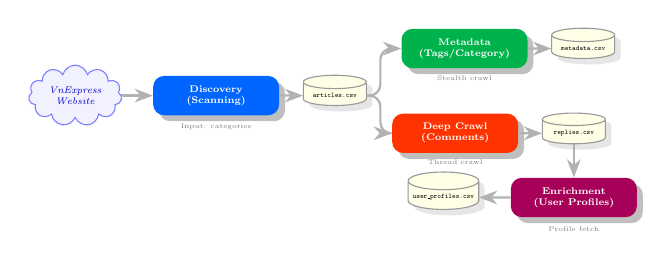
\begin{tikzpicture}[
  scale=0.5, transform shape,
  node distance=0.6cm and 0.9cm,
  process/.style={
    rectangle, rounded corners=4pt,
    minimum width=3.2cm, minimum height=1.0cm,
    align=center, text=white,
    font=\scriptsize\bfseries, drop shadow
  },
  step1/.style={process, fill=blue!60!cyan},
  step2/.style={process, fill=red!60!orange},
  step3/.style={process, fill=purple!60!violet},
  step4/.style={process, fill=teal!60!green},
  data/.style={
    cylinder, shape border rotate=90,
    draw=gray!80, fill=yellow!10, aspect=0.25,
    minimum height=0.75cm, minimum width=1.6cm,
    align=center, font=\tiny\ttfamily,
    drop shadow={opacity=0.2}
  },
  source/.style={
    cloud, cloud puffs=11,
    draw=blue!50, fill=blue!5, aspect=2,
    minimum width=2.0cm, minimum height=1.2cm,
    align=center, font=\scriptsize\itshape\color{blue!80!black}
  },
  arrow/.style={-Stealth, thick, draw=gray!60, rounded corners}
]
\node[source] (web) {VnExpress\\Website};

\node[step1, right=0.8cm of web] (s1) {Discovery\\(Scanning)};
\node[data, right=0.6cm of s1] (d1) {articles.csv};

\node[step4, above right=0.2cm and 1.2cm of d1] (s4) {Metadata\\(Tags/Category)};
\node[data, right=0.6cm of s4] (d4) {metadata.csv};

\node[step2, below right=0.2cm and 1.2cm of d1] (s2) {Deep Crawl\\(Comments)};
\node[data, right=0.6cm of s2] (d2) {replies.csv};

\node[step3, below=0.85cm of d2] (s3) {Enrichment\\(User Profiles)};
\node[data, left=0.8cm of s3] (d3) {user\_profiles.csv};

\draw[arrow] (web) -- (s1);
\draw[arrow] (s1) -- (d1);
\draw[arrow] (d1.east) -- ++(0.35,0) |- (s4.west);
\draw[arrow] (d1.east) -- ++(0.35,0) |- (s2.west);
\draw[arrow] (s4) -- (d4);
\draw[arrow] (s2) -- (d2);
\draw[arrow] (d2.south) -- (s3.north);
\draw[arrow] (s3) -- (d3);

\node[text=gray, font=\tiny, align=center, below=0.08cm of s1] {Input: categories};
\node[text=gray, font=\tiny, align=center, below=0.05cm of s4] {Stealth crawl};
\node[text=gray, font=\tiny, align=center, below=0.05cm of s2] {Thread crawl};
\node[text=gray, font=\tiny, align=center, below=0.1cm of s3] {Profile fetch};
\end{tikzpicture}
\caption{Pipeline thu thập dữ liệu và xuất các bảng trung gian phục vụ dựng đồ thị.}
\label{fig:crawler-pipeline}
\end{figure}

\subsection{Schema dữ liệu}
\tabref{tab:schema} tóm tắt schema 4 bảng dữ liệu sau chuẩn hóa.

\begin{table}[t]
\centering
\small
\setlength{\tabcolsep}{4pt}
\begin{tabular}{l p{5.6cm}}
\toprule
\textbf{Bảng} & \textbf{Trường chính}\\
\midrule
Articles & \texttt{article\_id, url, title, short\_description, author, published\_at, content}\\
Metadata & \texttt{article\_url, category, tags}\\
Replies & \texttt{article\_url, parent\_user\_id, parent\_text, ..., reply\_user\_id, reply\_text}\\
User Profiles & \texttt{user\_id, username, join\_date}\\
\bottomrule
\end{tabular}
\caption{Tóm tắt schema dữ liệu sau chuẩn hóa.}
\label{tab:schema}
\end{table}

\subsection{Thống kê tổng quan và độ thưa}
Dữ liệu sau thu thập gồm \textbf{3,645} bài viết, \textbf{15,693} người dùng và \textbf{40,045} tương tác (bình luận/trả lời). Trung bình có khoảng \textbf{2.55} tương tác mỗi user và \textbf{10.99} tương tác mỗi bài viết.

Độ thưa (sparsity) của ma trận tương tác user--article:
\begin{equation}
\text{Sparsity} = 1 - \frac{40{,}045}{15{,}693 \times 3{,}645} \approx 99.93\%.
\label{eq:sparsity}
\end{equation}
Mức độ thưa này cho thấy nguy cơ cold-start cao: đa số user có bậc nhỏ, gây khó khăn cho các mô hình thuần collaborative filtering.

\subsection{EDA: phân phối theo chuyên mục và hoạt động người dùng}
Các hình \figref{fig:eda-summary}--\figref{fig:eda-user-bottom} minh họa bức tranh tổng quan: phân phối chuyên mục, mức độ hoạt động của user và hiện tượng power-law (một nhóm nhỏ user đóng góp phần lớn tương tác).

\begin{figure}[t]
\centering
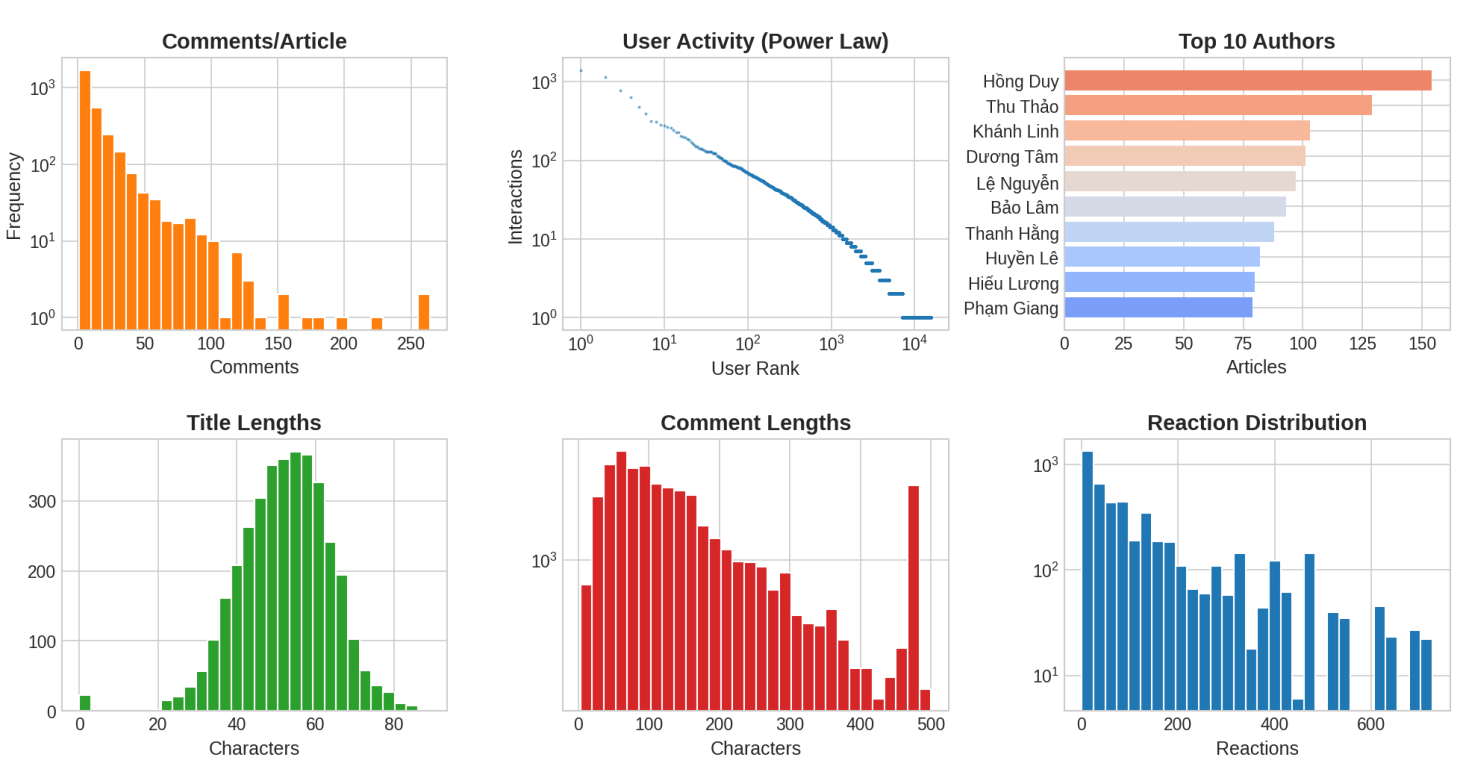
\includegraphics[width=\linewidth]{eda_00_summary_dashboard.png}
\caption{Dashboard tổng quan EDA.}
\label{fig:eda-summary}
\end{figure}

\begin{figure}[t]
\centering
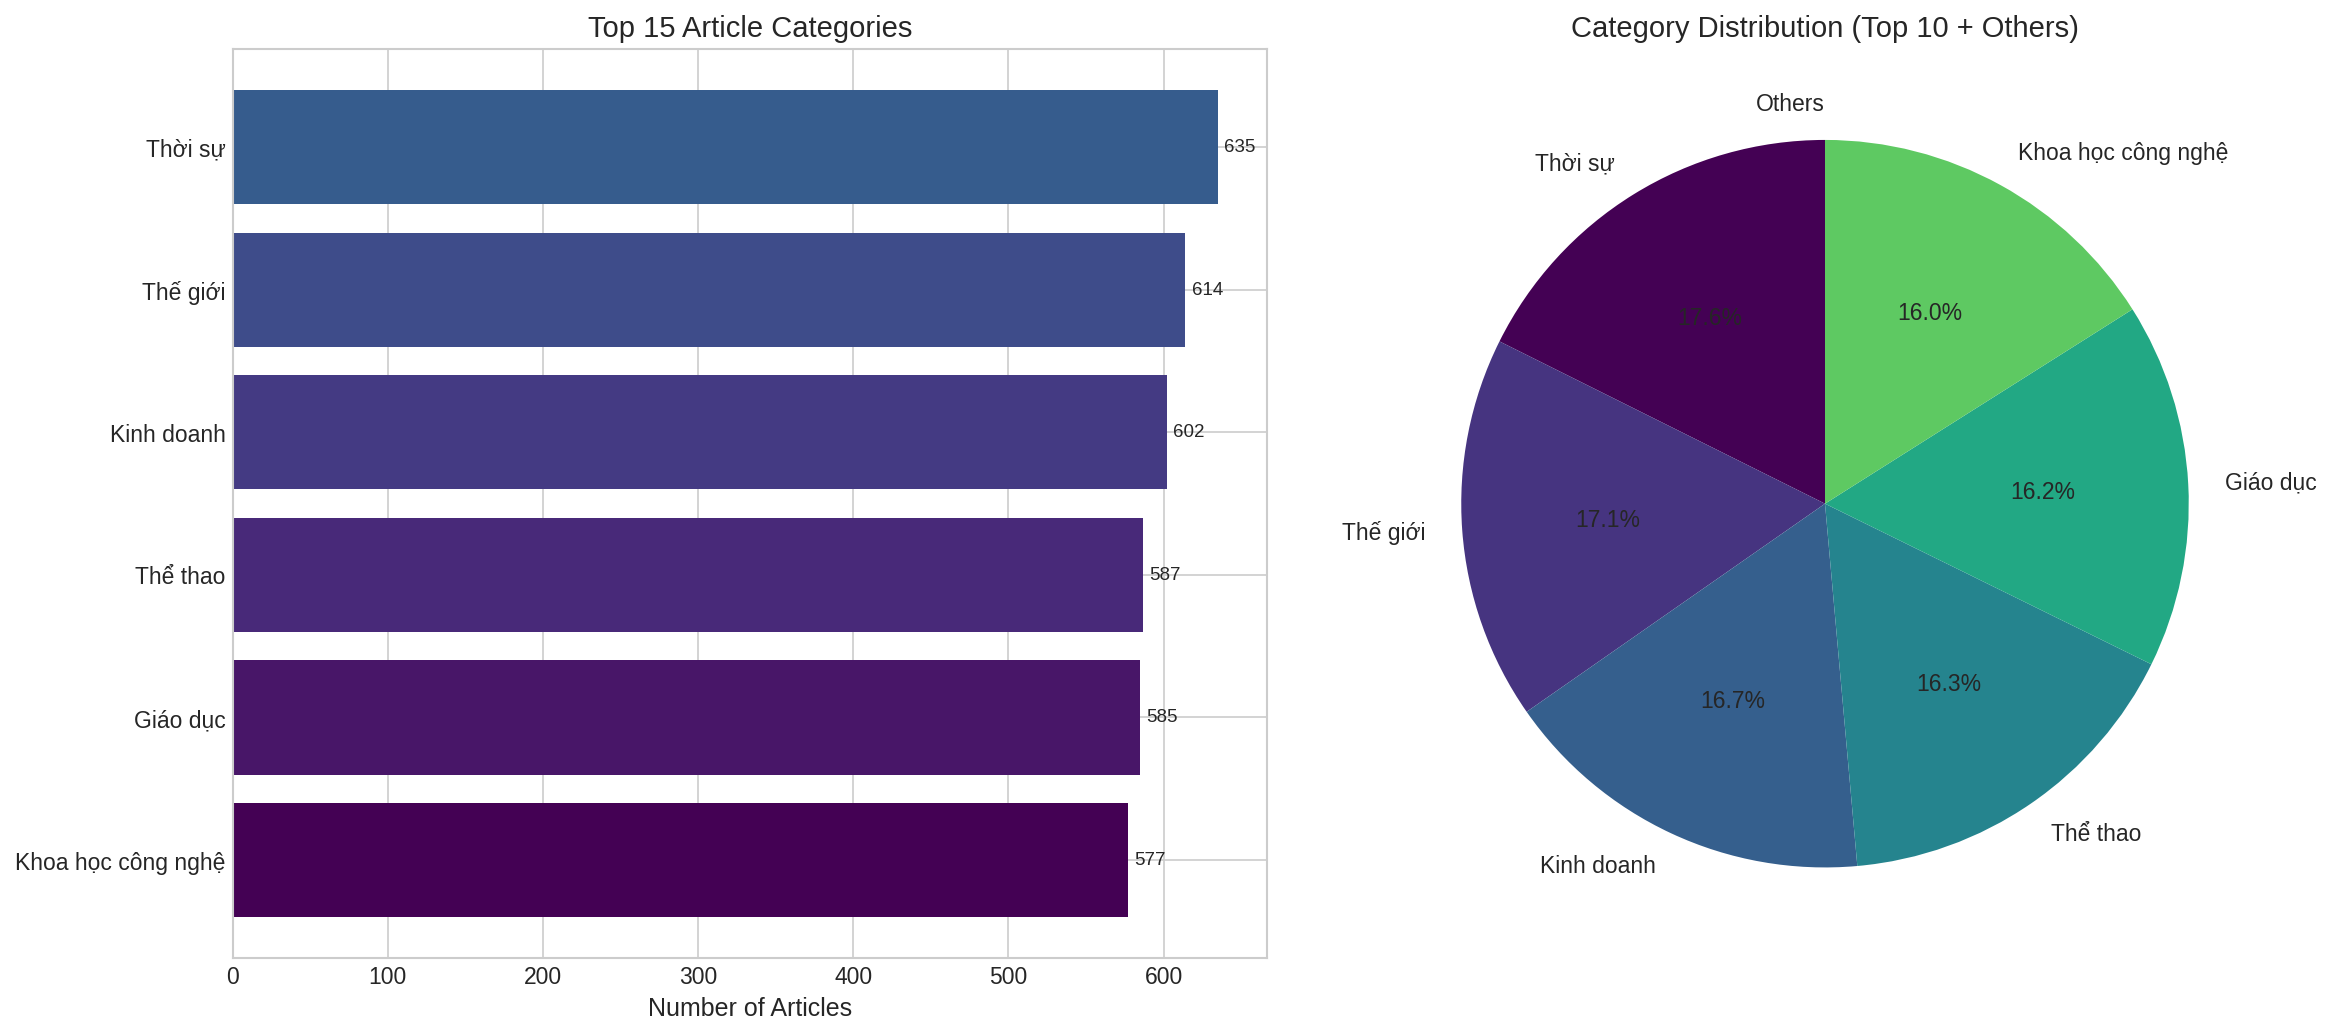
\includegraphics[width=\linewidth]{eda_09_metadata_categories.png}
\caption{Phân phối số bài theo chuyên mục.}
\label{fig:eda-category}
\end{figure}

\begin{figure}[t]
\centering
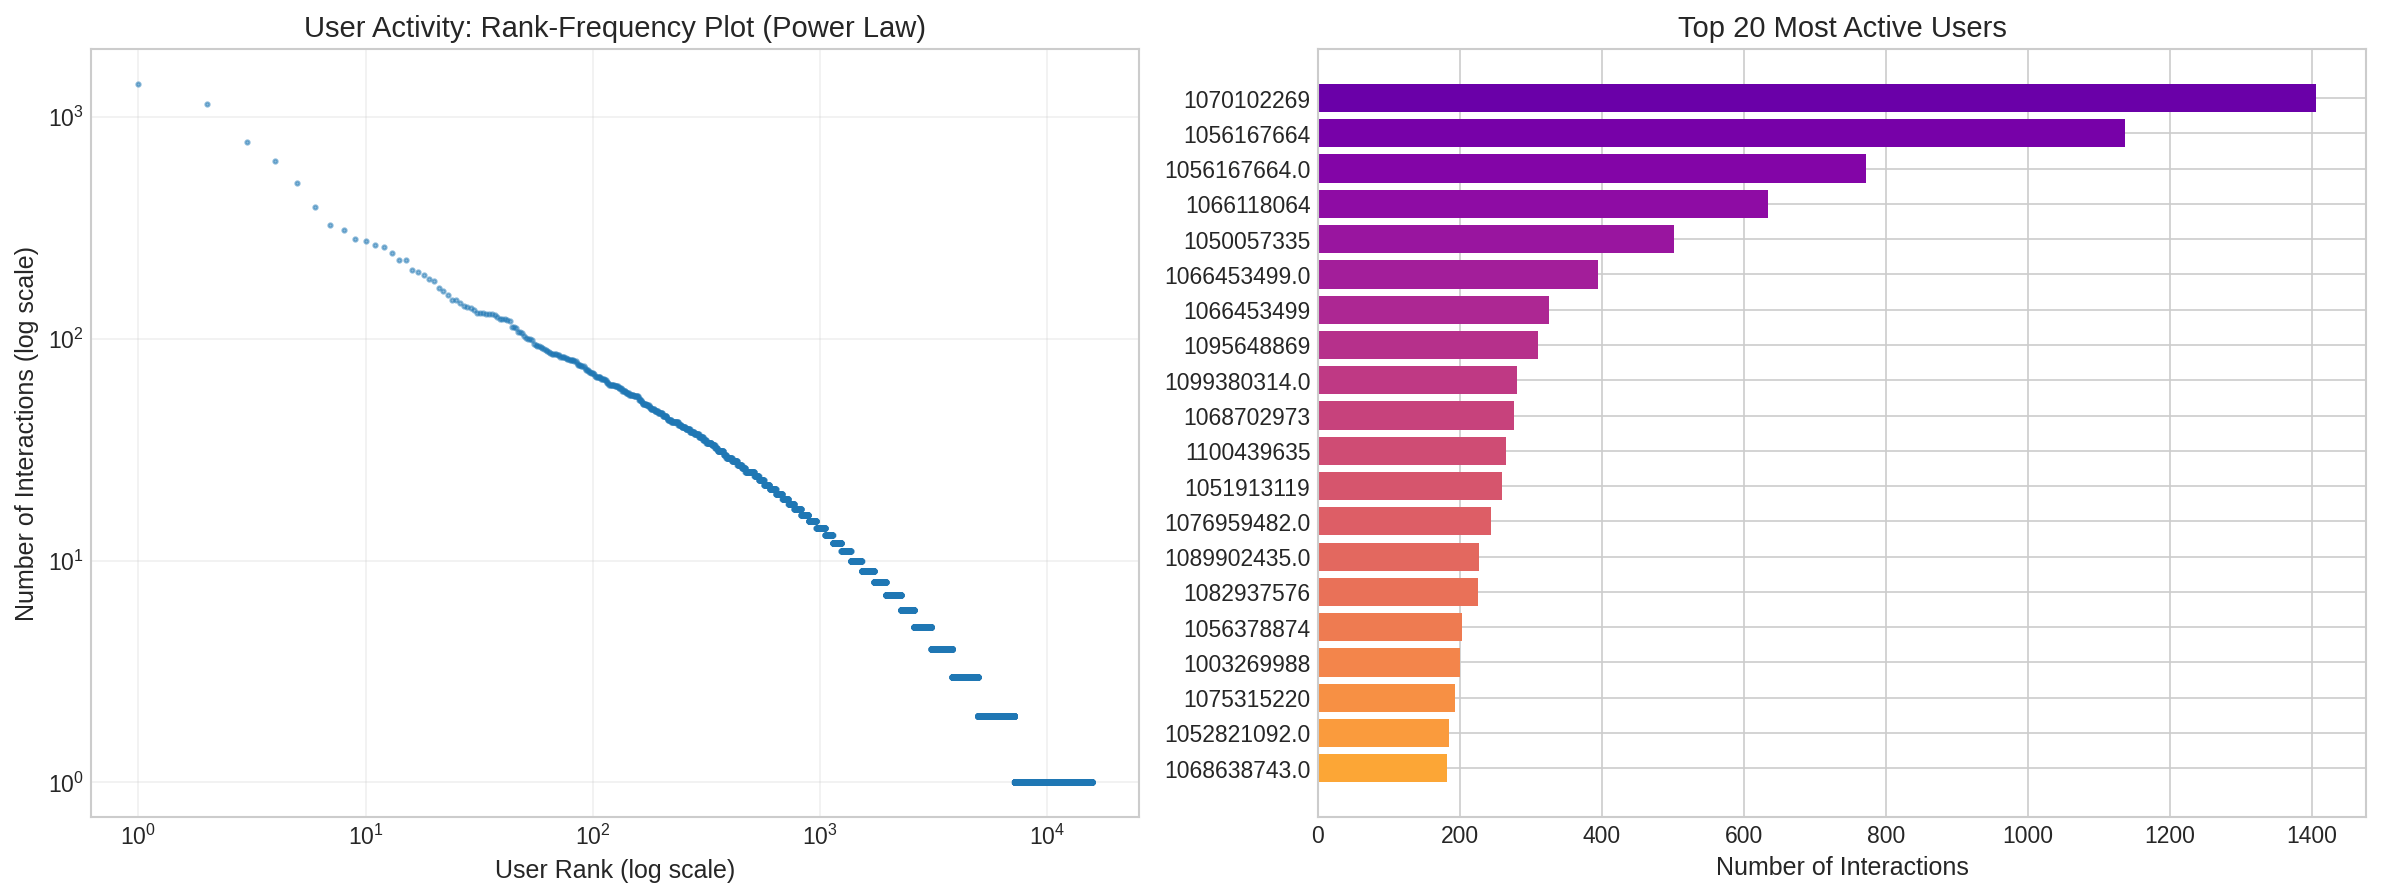
\includegraphics[width=\linewidth]{eda_03_user_activity_top.png}
\caption{Mẫu hình hoạt động người dùng (1/2).}
\label{fig:eda-user-top}
\end{figure}

\begin{figure}[t]
\centering
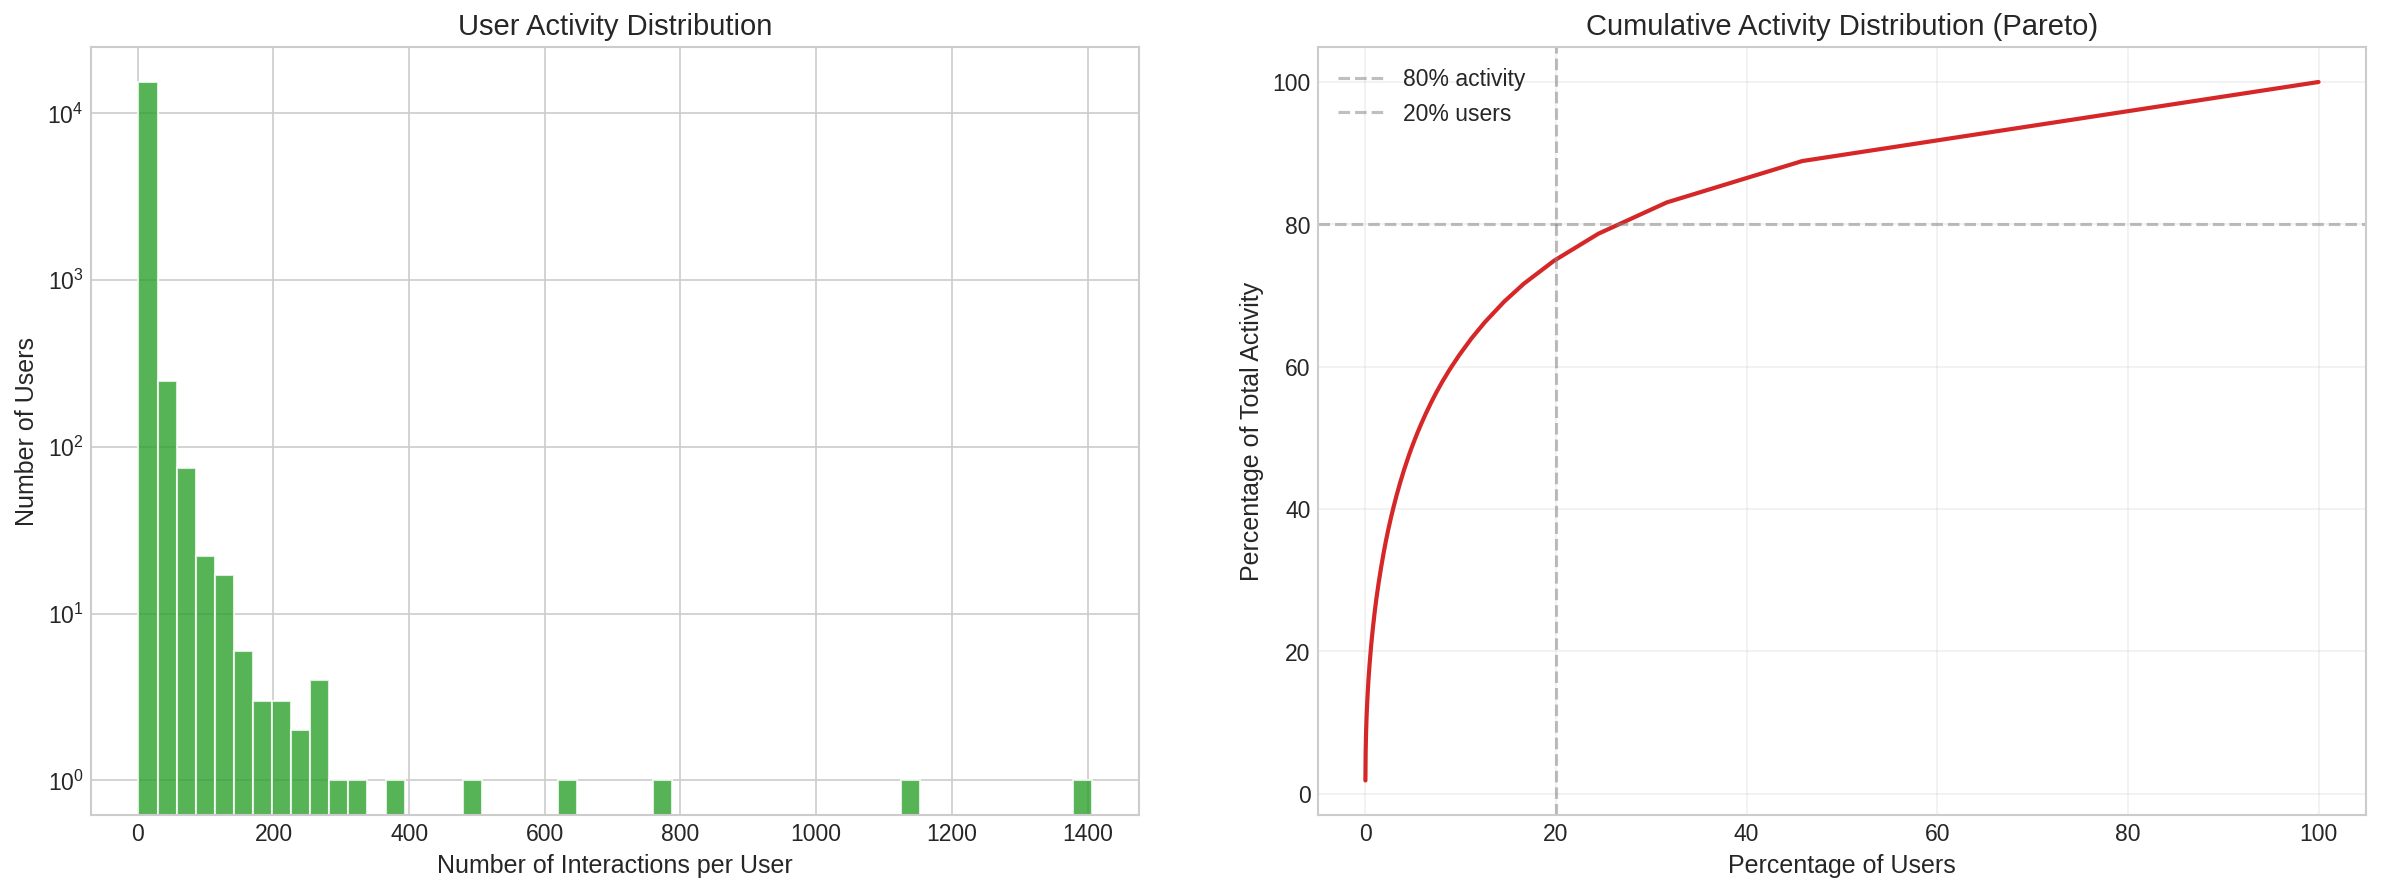
\includegraphics[width=\linewidth]{eda_03_user_activity_bottom.png}
\caption{Mẫu hình hoạt động người dùng (2/2): tương tác có xu hướng power-law.}
\label{fig:eda-user-bottom}
\end{figure}

\subsection{EDA: engagement theo chuyên mục và degree distribution}
\figref{fig:eda-eng-by-cat} mô tả mức độ tương tác theo chuyên mục. \figref{fig:degree} minh họa phân phối degree của user và article trong đồ thị tương tác; user degree thường nhỏ, phản ánh dữ liệu rất thưa.

\begin{figure}[t]
\centering
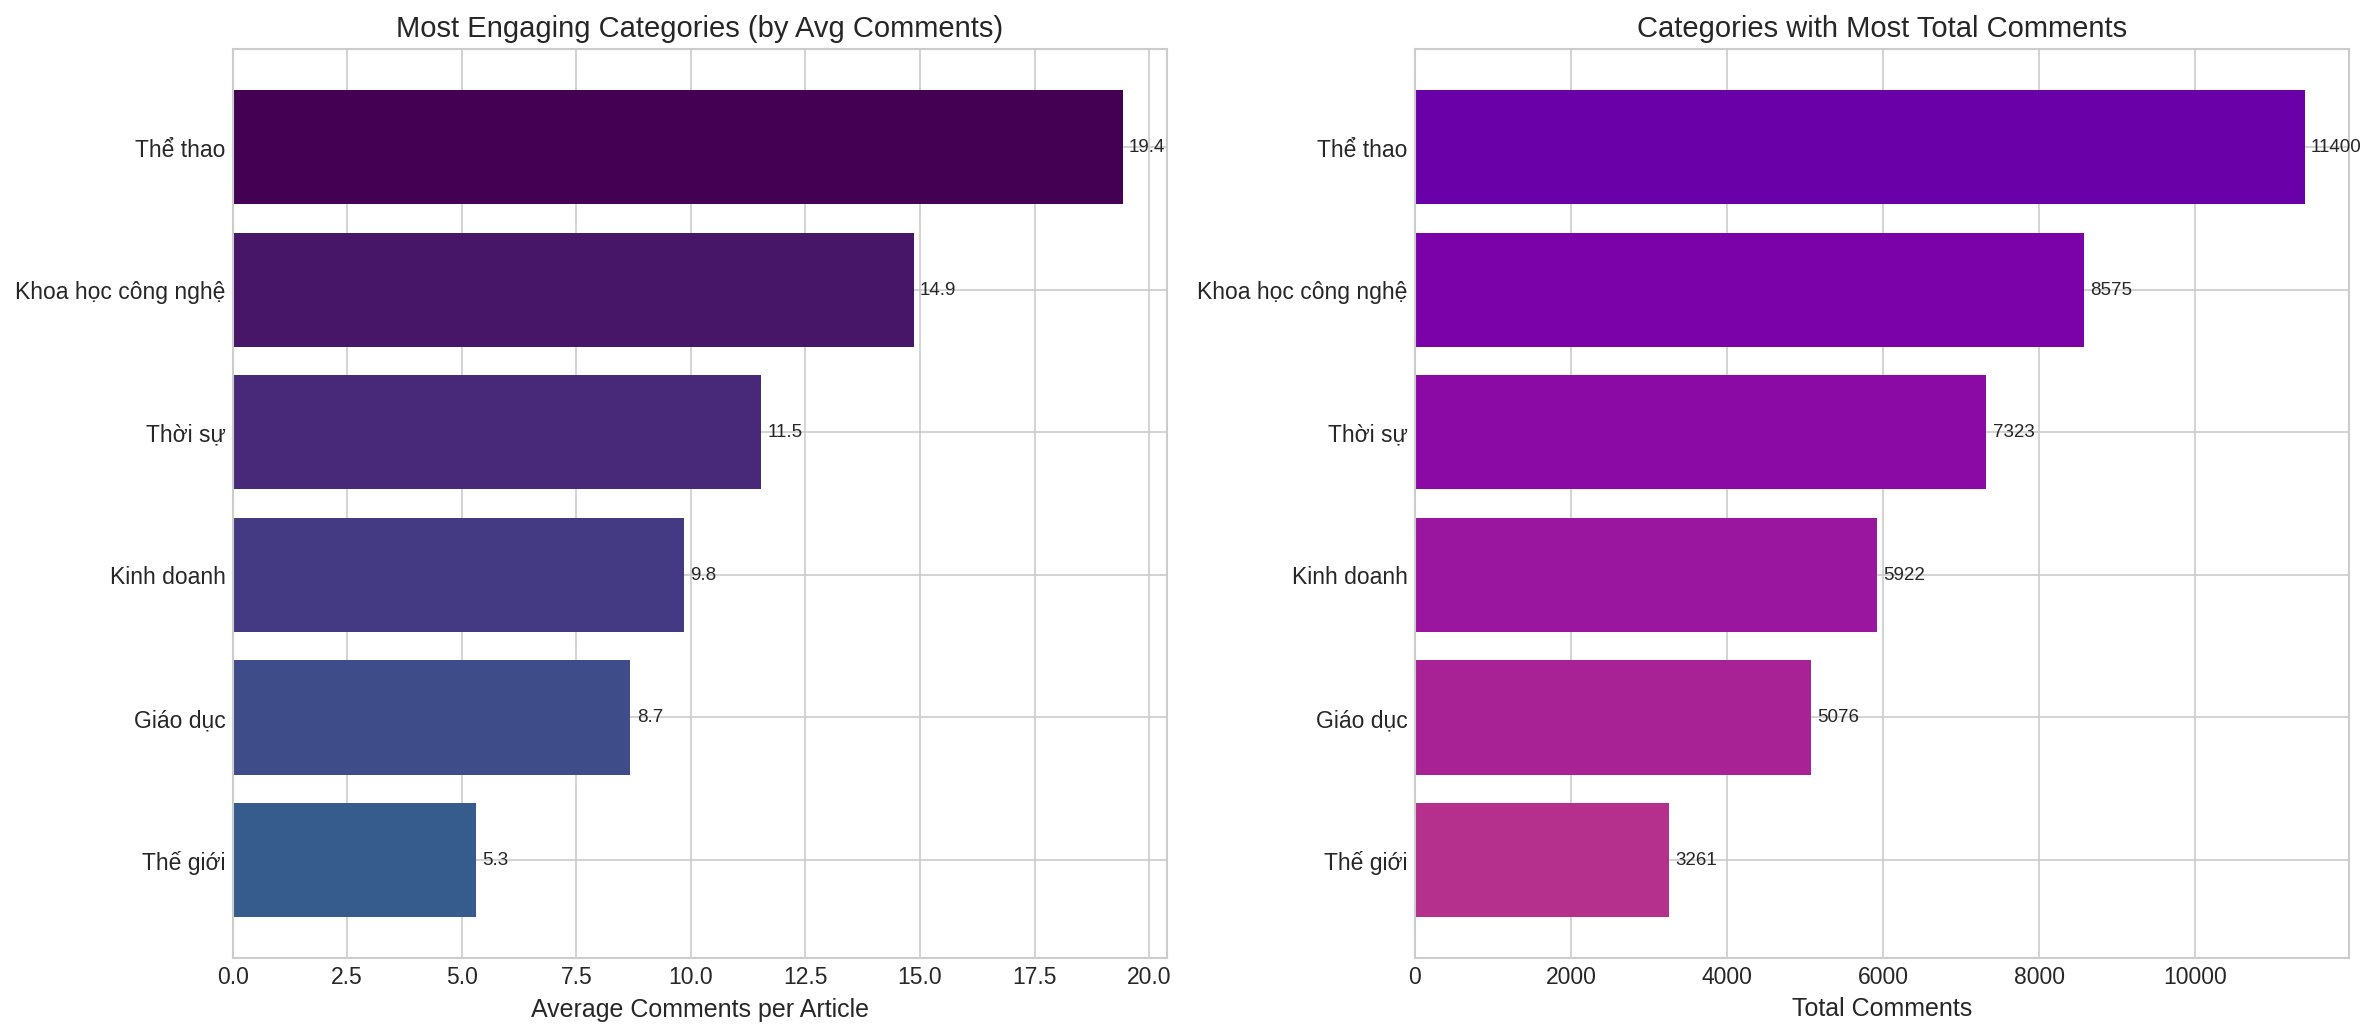
\includegraphics[width=\linewidth]{eda_11_engagement_by_category.png}
\caption{Tương tác theo chuyên mục.}
\label{fig:eda-eng-by-cat}
\end{figure}

\begin{figure}[t]
\centering
\begin{subfigure}{.49\linewidth}
  \centering
  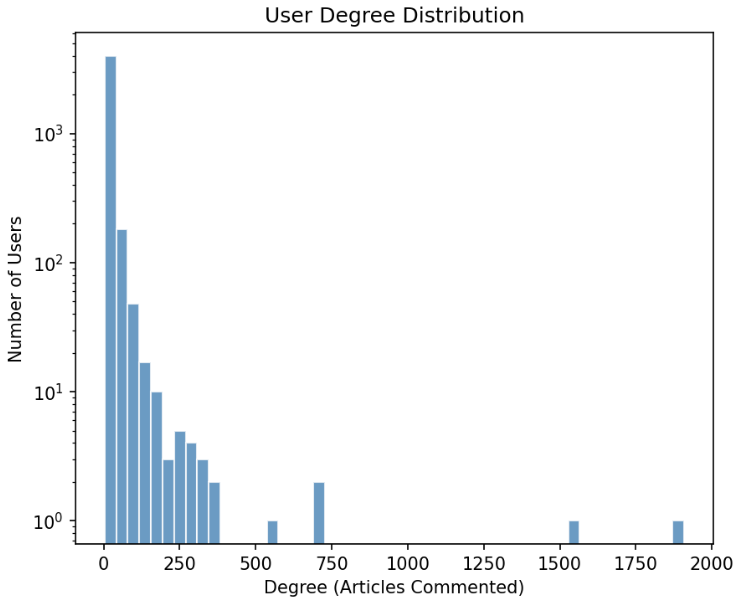
\includegraphics[width=\linewidth]{users_dis.png}
  \caption{Users}
\end{subfigure}
\begin{subfigure}{.49\linewidth}
  \centering
  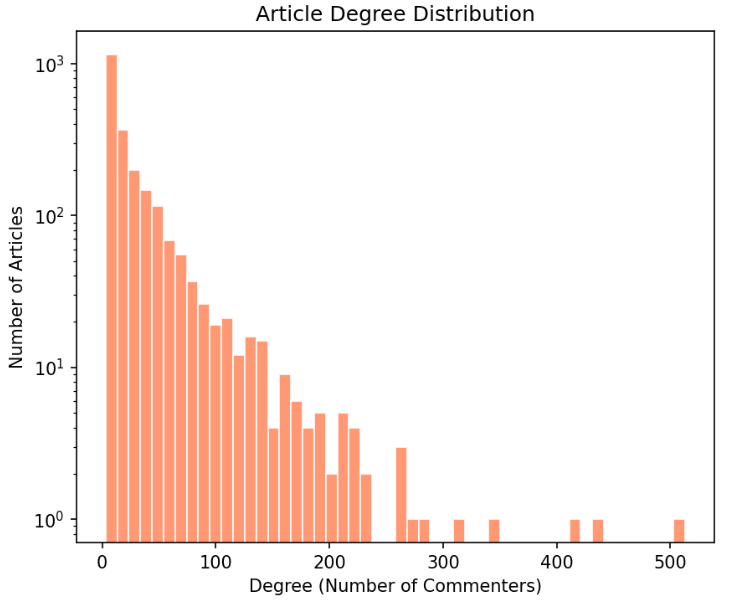
\includegraphics[width=\linewidth]{articles_dis.png}
  \caption{Articles}
\end{subfigure}
\caption{Phân phối degree trong đồ thị tương tác.}
\label{fig:degree}
\end{figure}

% ==========================================================
\section{Thiết kế đồ thị và chiến lược mở rộng (G1--G3)}
\label{sec:graph}

\subsection{Ý tưởng tổng quát}
Với sparsity rất cao (\eqref{eq:sparsity}), đồ thị user--article thuần túy khó lan truyền thông tin cho user ít tương tác. Do đó, chúng tôi thiết kế ba cấu trúc đồ thị tăng dần mức độ phong phú của tín hiệu:
\begin{itemize}
  \item \textbf{G1 (Bipartite):} chỉ gồm user và article với cạnh tương tác.
  \item \textbf{G2 (Social expansion):} bổ sung cạnh user--user từ quan hệ reply trong thảo luận.
  \item \textbf{G3 (Semantic hubs):} bổ sung node category để rút ngắn đường đi giữa user và nhóm bài cùng chuyên mục.
\end{itemize}

\subsection{Minh hoạ cấu trúc G1--G3}
\figref{fig:g123} minh họa trực quan sự khác nhau giữa ba đồ thị.

\begin{figure*}[t]
\centering
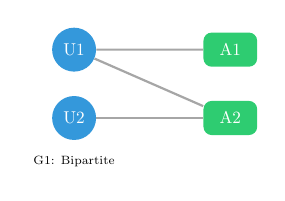
\begin{tikzpicture}[scale=0.62, transform shape]
\node[circle, fill=userblue, text=white, minimum size=0.9cm] (u1) at (0,1.4) {U1};
\node[circle, fill=userblue, text=white, minimum size=0.9cm] (u2) at (0,0) {U2};
\node[rectangle, rounded corners=3pt, fill=articlegreen, text=white, minimum width=1.1cm, minimum height=0.7cm] (a1) at (3.2,1.4) {A1};
\node[rectangle, rounded corners=3pt, fill=articlegreen, text=white, minimum width=1.1cm, minimum height=0.7cm] (a2) at (3.2,0) {A2};
\draw[-, thick, gray!70] (u1)--(a1);
\draw[-, thick, gray!70] (u1)--(a2);
\draw[-, thick, gray!70] (u2)--(a2);
\node[below=0.2cm of u2, font=\scriptsize] {G1: Bipartite};
\end{tikzpicture}
\hfill
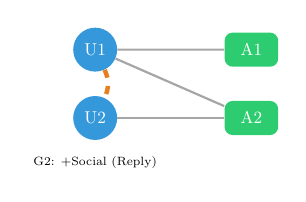
\begin{tikzpicture}[scale=0.62, transform shape]
\node[circle, fill=userblue, text=white, minimum size=0.9cm] (u1) at (0,1.4) {U1};
\node[circle, fill=userblue, text=white, minimum size=0.9cm] (u2) at (0,0) {U2};
\node[rectangle, rounded corners=3pt, fill=articlegreen, text=white, minimum width=1.1cm, minimum height=0.7cm] (a1) at (3.2,1.4) {A1};
\node[rectangle, rounded corners=3pt, fill=articlegreen, text=white, minimum width=1.1cm, minimum height=0.7cm] (a2) at (3.2,0) {A2};
\draw[-, thick, gray!70] (u1)--(a1);
\draw[-, thick, gray!70] (u1)--(a2);
\draw[-, thick, gray!70] (u2)--(a2);
\draw[-, dashed, ultra thick, socialorange, bend left=25] (u1) to (u2);
\node[below=0.2cm of u2, font=\scriptsize] {G2: +Social (Reply)};
\end{tikzpicture}

\vspace{0.2cm}

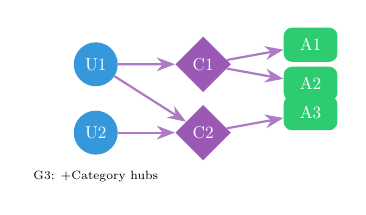
\begin{tikzpicture}[scale=0.62, transform shape]
\node[circle, fill=userblue, text=white, minimum size=0.9cm] (u1) at (0,1.4) {U1};
\node[circle, fill=userblue, text=white, minimum size=0.9cm] (u2) at (0,0) {U2};
\node[diamond, fill=cathub, text=white, minimum size=1.0cm] (c1) at (2.2,1.4) {C1};
\node[diamond, fill=cathub, text=white, minimum size=1.0cm] (c2) at (2.2,0) {C2};
\node[rectangle, rounded corners=3pt, fill=articlegreen, text=white, minimum width=1.1cm, minimum height=0.7cm] (a1) at (4.4,1.8) {A1};
\node[rectangle, rounded corners=3pt, fill=articlegreen, text=white, minimum width=1.1cm, minimum height=0.7cm] (a2) at (4.4,1.0) {A2};
\node[rectangle, rounded corners=3pt, fill=articlegreen, text=white, minimum width=1.1cm, minimum height=0.7cm] (a3) at (4.4,0.4) {A3};
\draw[-Stealth, thick, cathub!80] (u1)--(c1);
\draw[-Stealth, thick, cathub!80] (u1)--(c2);
\draw[-Stealth, thick, cathub!80] (u2)--(c2);
\draw[-Stealth, thick, cathub!80] (c1)--(a1);
\draw[-Stealth, thick, cathub!80] (c1)--(a2);
\draw[-Stealth, thick, cathub!80] (c2)--(a3);
\node[below=0.2cm of u2, font=\scriptsize] {G3: +Category hubs};
\end{tikzpicture}
\caption{Minh họa ba tầng đồ thị G1--G3 (bipartite, social expansion, semantic hubs).}
\label{fig:g123}
\end{figure*}

\subsection{Tách theo thời gian để hạn chế leakage}
Với dữ liệu tin tức, tương tác có tính thời gian mạnh. Khi xây dựng tập train/test, việc đảm bảo train thuộc quá khứ và test thuộc tương lai giúp mô phỏng đúng bối cảnh triển khai.

\begin{figure}[t]
\centering
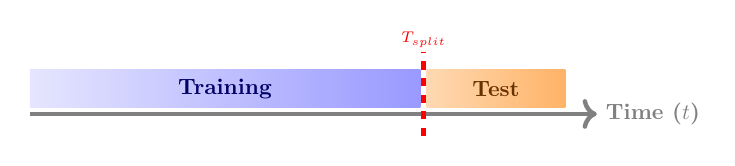
\begin{tikzpicture}[scale=0.8, transform shape]
\draw[->, ultra thick, gray] (0,0) -- (9,0) node[right, font=\bfseries] {Time ($t$)};
\shade[left color=blue!10, right color=blue!40] (0,0.1) rectangle (6.2,0.7);
\node[blue!40!black] at (3.1, 0.4) {\textbf{Training}};
\shade[left color=orange!30, right color=orange!60] (6.3,0.1) rectangle (8.5,0.7);
\node[orange!40!black] at (7.4, 0.4) {\textbf{Test}};
\draw[dashed, red, ultra thick] (6.25, -0.35) -- (6.25, 1.05);
\node[red, font=\bfseries\scriptsize, fill=white, inner sep=2pt] at (6.25, 1.18) {$T_{split}$};
\end{tikzpicture}
\caption{Minh họa tách train/test theo thời gian.}
\label{fig:temporal-split}
\end{figure}

% ==========================================================
\section{Phương pháp}
\label{sec:method}

\subsection{Bài toán và ký hiệu}
Gọi $U$ là tập người dùng, $A$ là tập bài viết. Mục tiêu là dự đoán mức phù hợp giữa user $u$ và article $a$ dựa trên lịch sử tương tác, sau đó xếp hạng và đề xuất Top-$K$ bài mà user chưa tương tác.

\subsection{Baseline đồ thị}
\paragraph{LightGCN.}
LightGCN lan truyền embedding tuyến tính theo adjacency chuẩn hóa:
\[
\mathbf{E}^{(k)} = \hat{\mathbf{A}} \mathbf{E}^{(k-1)}, \quad
\mathbf{E}^{*}=\sum_{k=0}^{K}\alpha_k \mathbf{E}^{(k)}.
\]
Đây là baseline hiệu quả cho recommendation trên đồ thị tương tác.

\paragraph{SimGCL / XSimGCL / LightGCL.}
Nhóm mô hình contrastive thêm ràng buộc InfoNCE để tạo embedding ổn định hơn trong dữ liệu thưa. SimGCL thêm nhiễu/perturbation trong quá trình propagation. XSimGCL tối giản hóa thiết kế để giảm chi phí nhưng vẫn duy trì lợi ích từ CL. LightGCL bổ sung thông tin global context nhằm vượt hạn chế chỉ dựa vào lân cận cục bộ.

\subsection{HGN: Heterogeneous GNN đa-aspect}
Dữ liệu chứa ít nhất hai quan hệ khác nhau: tương tác user--article (sở thích) và reply user--user (xã hội). HGN tách lan truyền thành hai nhánh:
\begin{itemize}
  \item \textbf{Interest path}: lan truyền trên $\mathcal{G}_{u-a}$.
  \item \textbf{Social path}: lan truyền trên $\mathcal{G}_{u-u}$.
\end{itemize}
Sau đó hợp nhất bằng phép cộng:
\begin{equation}
\mathbf{h}_u = \mathbf{h}_{int} + \mathbf{h}_{soc}.
\label{eq:fusion}
\end{equation}
Thiết kế này giúp tránh trộn lẫn ý nghĩa quan hệ, đồng thời giữ pipeline đơn giản để huấn luyện trên dữ liệu tương đối thưa.

\subsection{HCL: thử nghiệm heterogeneous contrastive learning}
HCL kết hợp heterogeneity (tách nhánh) và contrastive loss. Trong dữ liệu thưa, contrastive learning có thể nhạy với negative sampling và nhiệt độ (temperature), dẫn đến dao động trong huấn luyện. Chúng tôi giữ HCL như một thử nghiệm để quan sát và so sánh độ ổn định.

% ==========================================================
\section{Thiết lập thí nghiệm}
\label{sec:exp}

\subsection{Thiết lập huấn luyện}
Các mô hình được huấn luyện với 100 epochs, batch size 2048. Loss chính là BPR cho implicit feedback; các mô hình contrastive bổ sung InfoNCE.

\subsection{Protocol đánh giá}
\paragraph{Full Ranking (cold-start).}
Chia user theo tỉ lệ 80/20. Trên tập test, hệ thống xếp hạng các bài ứng viên và đo Recall@10, NDCG@10, Hit@10 và MRR.

\paragraph{Leave-One-Out (Loo100).}
Với mỗi user test, chọn 1 tương tác dương tính và 99 mẫu âm tính ngẫu nhiên để đánh giá chất lượng xếp hạng trong tập ứng viên nhỏ.

\subsection{Metric}
\begin{itemize}
  \item \textbf{Recall@10}: tỷ lệ thu hồi item đúng trong top-10.
  \item \textbf{Hit@10}: có/không item đúng trong top-10.
  \item \textbf{NDCG@10}: ưu tiên item đúng nằm ở vị trí cao.
  \item \textbf{MRR}: nhạy với vị trí item đúng đầu tiên.
\end{itemize}

% ==========================================================
\section{Kết quả và phân tích}
\label{sec:results}

\subsection{Kết quả Full Ranking}
\tabref{tab:full-ranking} tổng hợp kết quả theo từng đồ thị. Trong bối cảnh cold-start, baseline content-based thường có lợi thế vì dựa vào tương đồng ngữ nghĩa thay vì phụ thuộc hoàn toàn vào lịch sử tương tác. Đối với mô hình đồ thị, việc mở rộng G2 (thêm social edges) thường giúp lan truyền tín hiệu tốt hơn so với G1.

\begin{table*}[t]
\centering
\scriptsize
\setlength{\tabcolsep}{2.6pt}
\renewcommand{\arraystretch}{1.02}
\begin{tabularx}{\linewidth}{l|c|*4{>{\centering\arraybackslash}X}}
\toprule
\textbf{Model} & \textbf{Type} & \textbf{R@10} & \textbf{N@10} & \textbf{H@10} & \textbf{MRR}\\
\midrule
\multicolumn{6}{l}{\textit{\textbf{Content-Based / Baselines}}}\\
PhoBERT & CB & \textbf{0.0535} & \textbf{0.0315} & \textbf{0.0929} & \textbf{0.0416}\\
TF-IDF  & CB & 0.0508 & 0.0301 & 0.0951 & 0.0394\\
\midrule
\multicolumn{6}{l}{\textit{\textbf{Graph G1 (Bipartite)}}}\\
LightGCL & Graph CL & 0.0398 & 0.0249 & 0.0685 & 0.0313\\
LightGCN & Graph GNN& 0.0263 & 0.0145 & 0.0400 & 0.0174\\
XSimGCL  & Graph CL & \textbf{0.0439} & \textbf{0.0253} & \textbf{0.0694} & \textbf{0.0289}\\
HGN      & Hetero GNN & 0.0262 & 0.0147 & 0.0451 & 0.0182\\
HCL      & Hetero CL  & 0.0259 & 0.0164 & 0.0471 & 0.0214\\
SimGCL   & Graph CL & 0.0191 & 0.0115 & 0.0275 & 0.0135\\
\midrule
\multicolumn{6}{l}{\textit{\textbf{Graph G2 (User--User Social)}}}\\
LightGCL & Graph CL & \textbf{0.0436} & \textbf{0.0261} & \textbf{0.0739} & \textbf{0.0313}\\
LightGCN & Graph GNN& 0.0272 & 0.0156 & 0.0404 & 0.0186\\
XSimGCL  & Graph CL & 0.0432 & 0.0260 & 0.0688 & 0.0303\\
HGN      & Hetero GNN & 0.0369 & 0.0201 & 0.0596 & 0.0250\\
HCL      & Hetero CL  & 0.0320 & 0.0192 & 0.0520 & 0.0233\\
SimGCL   & Graph CL & 0.0228 & 0.0131 & 0.0312 & 0.0144\\
\midrule
\multicolumn{6}{l}{\textit{\textbf{Graph G3 (Category Hubs)}}}\\
LightGCL & Graph CL & \textbf{0.0413} & \textbf{0.0256} & \textbf{0.0710} & \textbf{0.0311}\\
LightGCN & Graph GNN& 0.0258 & 0.0145 & 0.0388 & 0.0175\\
XSimGCL  & Graph CL & 0.0379 & 0.0232 & 0.0643 & 0.0289\\
HGN      & Hetero GNN & 0.0299 & 0.0167 & 0.0464 & 0.0198\\
HCL      & Hetero CL  & 0.0250 & 0.0152 & 0.0471 & 0.0205\\
SimGCL   & Graph CL & 0.0222 & 0.0122 & 0.0322 & 0.0137\\
\bottomrule
\end{tabularx}
\caption{Kết quả Full Ranking cho ba cấu trúc đồ thị.}
\label{tab:full-ranking}
\end{table*}

\subsection{Kết quả Loo100}
Trong Loo100, HGN trên G2 đạt Recall@10 cao nhất, cho thấy việc tách social path và interest path giúp phân biệt dương/âm tốt hơn trong bối cảnh tập ứng viên nhỏ.

\begin{table*}[t]
\centering
\scriptsize
\setlength{\tabcolsep}{2.6pt}
\renewcommand{\arraystretch}{1.02}
\begin{tabularx}{\linewidth}{l|c|*4{>{\centering\arraybackslash}X}}
\toprule
\textbf{Model} & \textbf{Type} & \textbf{R@10} & \textbf{N@10} & \textbf{H@10} & \textbf{MRR}\\
\midrule
\multicolumn{6}{l}{\textit{\textbf{Graph G1 (Bipartite)}}}\\
LightGCL & Graph CL & \textbf{0.3081} & \textbf{0.2021} & \textbf{0.3822} & \textbf{0.2060}\\
LightGCN & Graph GNN& 0.2818 & 0.1743 & 0.3595 & 0.1782\\
XSimGCL  & Graph CL & 0.3009 & 0.1972 & 0.3787 & 0.2063\\
HGN      & Hetero GNN & 0.2740 & 0.1668 & 0.3570 & 0.1750\\
HCL      & Hetero CL  & 0.2047 & 0.1324 & 0.2802 & 0.1487\\
SimGCL   & Graph CL & 0.2129 & 0.1324 & 0.2920 & 0.1426\\
\midrule
\multicolumn{6}{l}{\textit{\textbf{Graph G2 (User--User Social)}}}\\
LightGCL & Graph CL & 0.3017 & 0.1986 & 0.3762 & 0.2034\\
LightGCN & Graph GNN& 0.2784 & 0.1727 & 0.3559 & 0.1778\\
XSimGCL  & Graph CL & 0.3036 & 0.2002 & 0.3827 & 0.2072\\
HGN      & Hetero GNN & \textbf{0.4364} & \textbf{0.2636} & \textbf{0.5155} & \textbf{0.2518}\\
HCL      & Hetero CL  & 0.2075 & 0.1355 & 0.2838 & 0.1546\\
SimGCL   & Graph CL & 0.2132 & 0.1322 & 0.2927 & 0.1434\\
\midrule
\multicolumn{6}{l}{\textit{\textbf{Graph G3 (Category Hubs)}}}\\
LightGCL & Graph CL & 0.3024 & 0.1988 & 0.3753 & 0.2022\\
LightGCN & Graph GNN& 0.2790 & 0.1697 & 0.3588 & 0.1733\\
XSimGCL  & Graph CL & 0.2969 & 0.1957 & 0.3726 & 0.2035\\
HGN      & Hetero GNN & \textbf{0.3127} & \textbf{0.1957} & \textbf{0.3896} & \textbf{0.1962}\\
HCL      & Hetero CL  & 0.2260 & 0.1492 & 0.2998 & 0.1631\\
SimGCL   & Graph CL & 0.2181 & 0.1333 & 0.2998 & 0.1435\\
\bottomrule
\end{tabularx}
\caption{Kết quả Leave-One-Out (Loo100) cho ba cấu trúc đồ thị.}
\label{tab:loo100}
\end{table*}

\subsection{Tác động topology và phân tích HGN}
Để định lượng tác động của mở rộng đồ thị lên HGN, \tabref{tab:impact-graph} so sánh Recall@10 của HGN theo từng cấu trúc. Kết quả cho thấy việc bổ sung social edges giúp tăng hiệu quả, trong khi category hubs có thể làm tín hiệu trở nên quá rộng.

\begin{table}[t]
  \centering
  \small
  \setlength{\tabcolsep}{3pt}
  \renewcommand{\arraystretch}{1.05}
  \begin{tabularx}{\linewidth}{l X c}
  \toprule
  \textbf{Graph} & \textbf{Thống kê cấu trúc} & \textbf{R@10 (HGN)}\\
  \midrule
  G1 & 13k Users, 30k Edges; Density: 0.06\% & 0.0262\\
  G2 & +61k Social Edges; Density: 0.064\% & \textbf{0.0369}\\
  G3 & +6 Categories; 16k User-Cat Edges; Density: 0.096\% & 0.0299\\
  \bottomrule
  \end{tabularx}
  \caption{Ảnh hưởng cấu trúc đồ thị lên HGN.}
  \label{tab:impact-graph}
\end{table}
  

\subsection{So sánh backbone cho HGN}
Chúng tôi khảo sát ba backbone (GAT, GraphSAGE, TransformerConv). TransformerConv đạt Recall@10 cao nhất trong thiết lập full protocol.

\begin{table}[t]
  \centering
  \small
  \setlength{\tabcolsep}{3pt}
  \begin{tabular}{l|cc|ccc}
  \toprule
  \textbf{Backbone} & \multicolumn{2}{c|}{\textbf{Full}} & \multicolumn{3}{c}{\textbf{Chi phí}}\\
   & R@10 & N@10 & Inf. (s) & Params & Train (s)\\
  \midrule
  GAT  & 0.0262 & 0.0163 & $\sim$1.38 & 1.27M & 20.23\\
  SAGE & 0.0303 & 0.0182 & $\sim$0.88 & 1.27M & 19.77\\
  TRANS & \textbf{0.0454} & \textbf{0.0236} & 1.71 & 1.47M & 19.76\\
  \bottomrule
  \end{tabular}
  \caption{So sánh backbone của HGN (TRANS = TransformerConv).}
  \label{tab:backbone}
\end{table}
  

\subsection{Ablation: edge types và độ sâu}
Loại bỏ social edges làm giảm Recall@10; loại bỏ category làm giảm mạnh hơn, cho thấy category cung cấp tín hiệu rộng nhưng hữu ích trong một số kịch bản.

\begin{table}[t]
  \centering
  \small
  \setlength{\tabcolsep}{4pt}
  \begin{tabular}{l|c|c|l}
  \toprule
  \textbf{Cấu hình} & \textbf{Recall@10} & \textbf{Giảm (\%)} & \textbf{Gợi ý}\\
  \midrule
  G2 (full) & \textbf{0.0369} & -- & Best\\
  w/o social & 0.0293 & -20.6\% & Social signal\\
  w/o cat. & 0.0227 & -38.5\% & Semantic hub\\
  \bottomrule
  \end{tabular}
  \caption{Ablation theo loại cạnh/đường đi (cat.\ = category).}
  \label{tab:ablation-metapath}
\end{table}
  

Độ sâu lan truyền $L$ cho thấy LightGCN giảm hiệu quả khi tăng $L$ do over-smoothing, trong khi LightGCL/XSimGCL ổn định hơn.

\begin{table}[t]
\centering
\small
\begin{tabularx}{\linewidth}{l|*4{>{\centering\arraybackslash}X}}
\toprule
\textbf{Model} & \textbf{L=1} & \textbf{L=2} & \textbf{L=3} & \textbf{L=4}\\
\midrule
LightGCL & 0.032 & 0.040 & 0.043 & 0.042\\
XSimGCL  & 0.028 & 0.035 & 0.039 & 0.041\\
LightGCN & 0.031 & 0.026 & 0.022 & 0.019\\
HGN      & 0.033 & 0.032 & 0.026 & 0.028\\
HCL      & 0.020 & 0.010 & 0.007 & 0.009\\
SimGCL   & 0.024 & 0.027 & 0.021 & 0.023\\
\bottomrule
\end{tabularx}
\caption{Ablation theo độ sâu lan truyền $L$.}
\label{tab:ablation-depth}
\end{table}

\subsection{Phân tích chi phí huấn luyện}
XSimGCL có thời gian/epoch nhanh nhất trong thiết lập so sánh. Mô hình heterogeneous có thể tốn chi phí hơn khi đồ thị dày hơn do mở rộng social.

\begin{table}[t]
  \centering
  \footnotesize
  \setlength{\tabcolsep}{3pt}
  \renewcommand{\arraystretch}{1.05}
  \begin{tabular}{l|c|ccc}
  \toprule
  \textbf{Model} & \textbf{Params} & \textbf{G1} & \textbf{G2} & \textbf{G3}\\
  \midrule
  SimGCL   & 1.07M & 00:47 & 00:46 & 00:45\\
  XSimGCL  & 1.07M & \textbf{00:35} & \textbf{00:33} & \textbf{00:34}\\
  LightGCL & 1.07M & 00:46 & 00:45 & 00:45\\
  \midrule
  HCL & 1.07M & 00:47 & 01:10 & 00:37\\
  HGN & 1.27M & 01:29 & 02:23 & 00:35\\
  \bottomrule
  \end{tabular}
  \caption{Chi phí huấn luyện (phút:giây) và số tham số theo cấu hình thí nghiệm.}
\label{tab:efficiency}
\end{table}
  

% ==========================================================
\section{Thảo luận}
\label{sec:discussion}

\subsection{Vì sao mở rộng social (G2) hữu ích?}
Social edges tăng kết nối giữa người dùng ngay cả khi họ không tương tác cùng bài viết, giúp lan truyền embedding tốt hơn trong dữ liệu thưa. Với thiết kế dual-path, tín hiệu xã hội được khai thác mà không làm nhiễu tín hiệu sở thích trực tiếp.

\subsection{Vì sao category hubs (G3) có thể không ổn định?}
Category mang tính khái quát. Khi liên kết user với category và category với nhiều bài viết, mô hình có thể ưu tiên các gợi ý ``cùng chuyên mục'' nhưng kém cá nhân hóa, dẫn đến over-generalization trong một số thiết lập.

\subsection{Vì sao HCL dễ dao động?}
Trong regime thưa, số positive ít và negative sampling nhạy cảm khiến InfoNCE khó ổn định. Khi kết hợp thêm heterogeneity (hai nhánh lan truyền), việc cân bằng loss và hyper-parameter trở nên khó hơn, dẫn đến hiện tượng khó hội tụ ổn định.

% ==========================================================
\section{Kết luận và hướng phát triển}
\label{sec:conclusion}

\subsection{Kết luận}
Báo cáo xây dựng hệ gợi ý bài báo tiếng Việt dựa trên học đồ thị từ dữ liệu VnExpress: pipeline thu thập, EDA, ba cấu trúc đồ thị G1--G3, benchmark các mô hình đồ thị hiện đại và thử nghiệm heterogeneous. Kết quả chỉ ra rằng mở rộng social graph giúp cải thiện đáng kể cho mô hình heterogeneous; trong khi đó, content-based vẫn là thành phần quan trọng trong bối cảnh cold-start.

\subsection{Hạn chế}
\begin{itemize}
  \item Dữ liệu dựa trên bình luận/trả lời có thể thiên lệch vì nhiều lượt đọc không tạo tương tác.
  \item Chi phí huấn luyện tăng khi đồ thị mở rộng, đặc biệt với mô hình heterogeneous.
  \item Mô hình hiện tại là static, chưa xử lý cập nhật online khi tin mới xuất hiện.
\end{itemize}

\subsection{Hướng phát triển}
\begin{itemize}
  \item Học đồ thị động để nắm bắt sự thay đổi sở thích theo thời gian.
  \item Mở rộng meta-path bằng tags/author/entity để tăng mức độ ngữ nghĩa chi tiết hơn category.
  \item Thiết kế self-supervised learning ổn định hơn trong dữ liệu cực thưa.
  \item Distillation/nén mô hình để giảm chi phí inference khi triển khai.
\end{itemize}

% ==========================================================
\section*{Tài liệu tham khảo}
\FloatBarrier
\bibliography{references}

\end{document}
